{
\newcommand{\figWidtha}{5.5cm}
\newcommand{\trimfiga}[2]{\trimPlotb{#1}{#2}{.1}{.2}{.075}{.15}}
% \newcommand{\cbWidth}{7.cm}
% \newcommand{\clipfigcb}[2]{\clipFig{#1}{#2}{.881}{.918}{.118}{.885}}
\begin{figure}[hbt]
\begin{center}
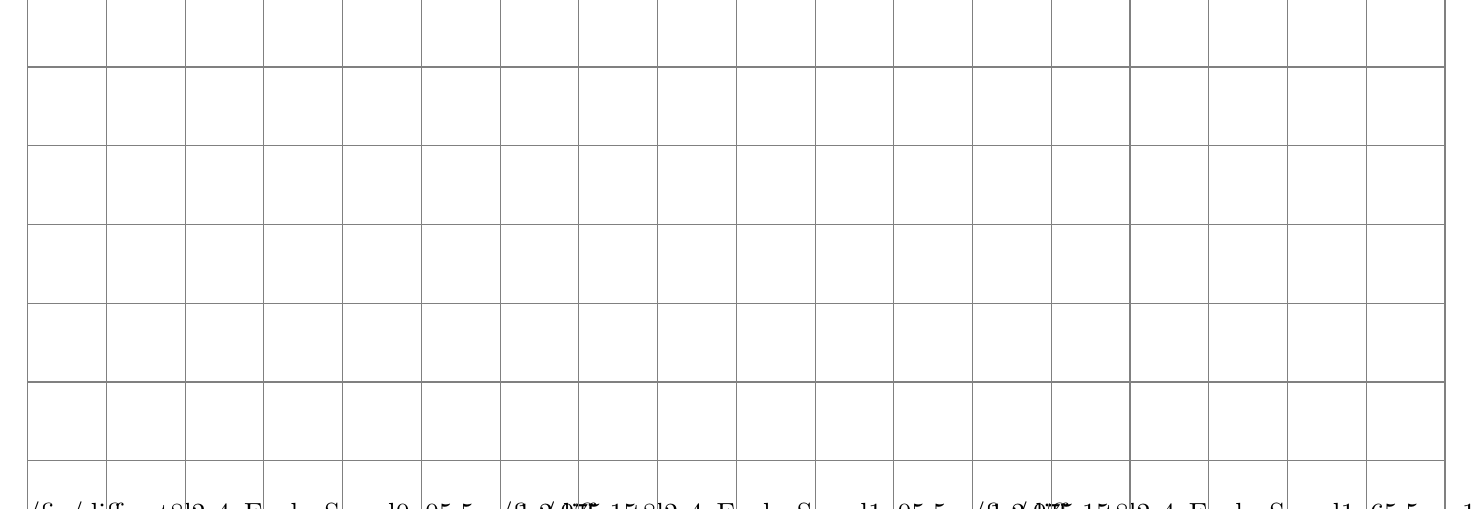
\begin{tikzpicture}[scale=1]
  \useasboundingbox (0,.75) rectangle (18.0,6.5);  % set the bounding box (so we have less surrounding white spa  
  \draw ( 0.0,0.0) node[anchor=south west,xshift=-4pt,yshift=+0pt] {\trimfiga{\smDocDir/fig/diffract8l2r4gEvolveSpeed0p0}{\figWidtha}};
  \draw ( 6.0,0.0) node[anchor=south west,xshift=-4pt,yshift=+0pt] {\trimfiga{\smDocDir/fig/diffract8l2r4gEvolveSpeed1p0}{\figWidtha}};
  \draw (12.0,0.0) node[anchor=south west,xshift=-4pt,yshift=+0pt] {\trimfiga{\smDocDir/fig/diffract8l2r4gEvolveSpeed1p6}{\figWidtha}};
% grid:
  \draw[step=1cm,gray] (0,0) grid (18,7.);
\end{tikzpicture}
%+\begin{pspicture}(0,.75)(16.0,5.45)
%+ \rput(2.5 , 3.0){\clipfig{diffract/diffract8l2r4gEvolveSpeed0p0.ps}{\figWidth}}
%+ \rput( 7.6, 3.0){\clipfig{diffract/diffract8l2r4gEvolveSpeed1p0.ps}{\figWidth}}
%+ \rput(12.7, 3.0){\clipfig{diffract/diffract8l2r4gEvolveSpeed1p6.ps}{\figWidth}}
%+% 
%+% -- colour bar --
%+\rput(15.25,2.80){%
%+\rput(-3.0,0.){\clipfigcb{colourBarLines.ps}{\cbWidth}}
%+\rput(.72,0.){\rput[l](-.45,2.55){\smallss }\rput[l](-.45,-2.5){\smallss }\rput(-.25,0){\smallss $\vert \vv\vert$}}
%+% \rput(.72,0.){\rput[l](-.45,2.55){\smallss 2.4}\rput[l](-.45,-2.5){\smallss 0.0}\rput(-.25,0){\smallss $\vert \vv\vert$}}
%+}
%+% \psgrid[subgriddiv=2]
%+\end{pspicture}
\end{center}
\caption{Diffraction of a p-wave shock by a circular cavity.  Numerical solution computed with AMR using one refinement level with $n_r=4$ and
the FOS scheme.  Shaded contours of the magnitude of velocity at times (from left to right)
$t=0$ (contour bounds $[0,1.82]$), $t=1.0$ ($[0,2.79]$) and $t=1.6$ ($[0,2.41]$).
The boundaries of the base-level component grids are shown in blue and the boundaries of the refinement grids are shown in green.  The deformed grid is shown using a scaling of the displacement by a factor of $0.075$. }
\label{fig:cylDiffractEvolution}
\end{figure}
}
